\documentclass{exam}
\usepackage[utf8]{inputenc}
\usepackage{lmodern}
\usepackage{microtype}

% \usepackage[parfill]{parskip}
\usepackage[dvipsnames]{xcolor}
\usepackage{amsmath}
\usepackage{amsfonts}
\usepackage{amsthm}
\usepackage{siunitx}
\DeclareSIUnit\year{yr}
\DeclareSIUnit\foot{ft}
\DeclareSIUnit\litre{\liter}

\usepackage{skull}

\usepackage{pgfplots}
\usepgfplotslibrary{polar}
\pgfplotsset{compat=1.11}
\usepgfplotslibrary{statistics}
\usepackage{graphicx}
\usepackage{sidecap}
\sidecaptionvpos{figure}{c}
\usepackage{float}
\usepackage{gensymb}
\usepackage{tkz-euclide}
\usetkzobj{all}
\usepackage{commath}
\usepackage{hyperref}
\usepackage{enumitem}
\usepackage{wasysym}
\usepackage{multicol}
\usepackage{mathtools}
\usepackage{tcolorbox}
\usepackage{tabularx}
\usepackage[version=4]{mhchem}
\usepackage{changepage}
\usepackage{listings}
\lstset{basicstyle=\ttfamily\linespread{0.8}\small}

\renewcommand*{\thefootnote}{\fnsymbol{footnote}}

\newtheorem*{thm}{Theorem}
\newtheorem*{iden}{Identity}
\newtheorem*{lemma}{Lemma}
\newtheorem{obs}{Observation}
\theoremstyle{definition}
\newtheorem*{defn}{Definition}
\newtheorem*{ex}{Example}
\newtheorem{con}{Construction}
\newtheorem*{alg}{Algorithm}

\newtheoremstyle{break}
  {\topsep}{\topsep}%
  {\itshape}{}%
  {\bfseries}{}%
  {\newline}{}%
\theoremstyle{break}
\newtheorem*{bthm}{Theorem}

% russian integral
\usepackage{scalerel}
\DeclareMathOperator*{\rint}{\scalerel*{\rotatebox{17}{$\!\int\!$}}{\int}}

% \DeclareMathOperator*{\rint}{\int}

\pgfplotsset{vasymptote/.style={
    before end axis/.append code={
        \draw[densely dashed] ({rel axis cs:0,0} -| {axis cs:#1,0})
        -- ({rel axis cs:0,1} -| {axis cs:#1,0});
    }
}}

% \pointsinrightmargin
\boxedpoints
\pointname{}

\newcommand{\questioA}{\question[\texttt{\textbf{\color{Cerulean} A}}]}
\newcommand{\questioM}{\question[\texttt{\textbf{\color{PineGreen} M}}]}
\newcommand{\questioE}{\question[\texttt{\textbf{\color{WildStrawberry} E}}]}
\newcommand{\questioS}{\question[\texttt{\textbf{\color{Goldenrod} S}}]}
\newcommand{\questioO}{\question[\texttt{\textbf{\color{BurntOrange} O}}]}

\newcommand{\parA}{\part[\texttt{\textbf{\color{Cerulean} A}}]}
\newcommand{\parM}{\part[\texttt{\textbf{\color{PineGreen} M}}]}
\newcommand{\parE}{\part[\texttt{\textbf{\color{WildStrawberry} E}}]}
\newcommand{\parS}{\part[\texttt{\textbf{\color{Goldenrod} S}}]}
\newcommand{\parO}{\part[\texttt{\textbf{\color{BurntOrange} O}}]}

\newcommand{\subparA}{\subpart[\texttt{\textbf{\color{Cerulean} A}}]}
\newcommand{\subparM}{\subpart[\texttt{\textbf{\color{PineGreen} M}}]}
\newcommand{\subparE}{\subpart[\texttt{\textbf{\color{WildStrawberry} E}}]}
\newcommand{\subparS}{\subpart[\texttt{\textbf{\color{Goldenrod} S}}]}
\newcommand{\subparO}{\subpart[\texttt{\textbf{\color{BurntOrange} O}}]}

\newcommand{\mainHeader}[2]{\section*{NCEA Level 2 Mathematics\\#1. #2}}
\newcommand{\mainHeaderHw}[2]{\section*{NCEA Level 2 Mathematics (Homework)\\#1. #2}}
\newcommand{\seealso}[1]{\begin{center}\emph{See also #1.}\end{center}}
\newcommand{\drills}[1]{\begin{center}\emph{Drill problems: #1.}\end{center}}
\newcommand{\basedon}[1]{\begin{center}\emph{Notes largely based on #1.}\end{center}}

\begin{document}

\mainHeaderIntgHw{23}{Trigonometric Substitution}
\subsection*{Reading}
\begin{center}
  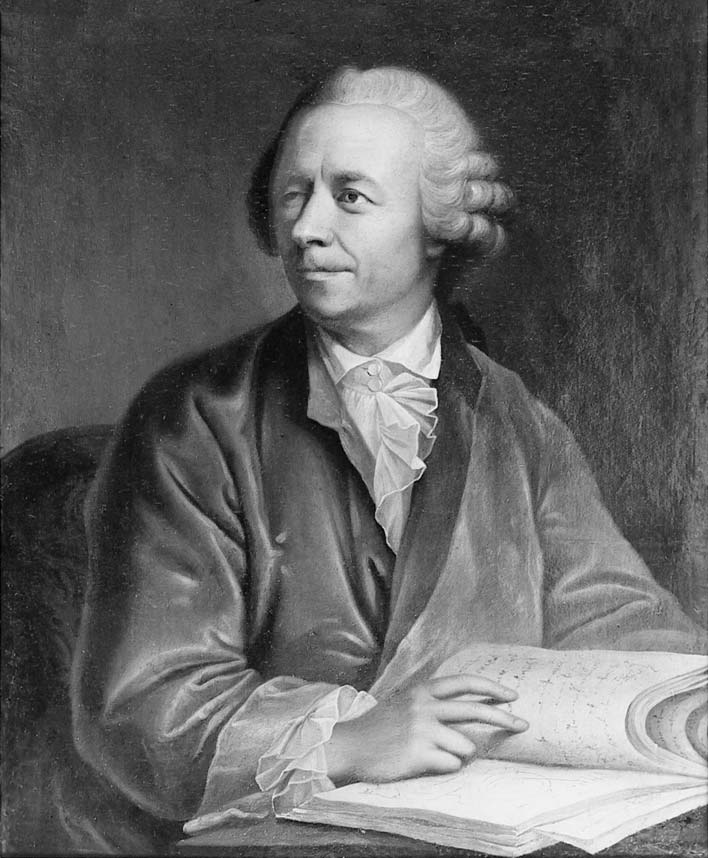
\includegraphics[width=0.2\textwidth]{euler}
\end{center}
Leonhard Euler, (born April 15, 1707, Basel, Switzerland --- died September 18, 1783, St. Petersburg, Russia), Swiss mathematician and physicist, one of the founders of pure mathematics. He not only made decisive and formative contributions to the subjects of geometry, calculus, mechanics, and number theory but also developed methods for solving problems in observational astronomy and demonstrated useful applications of mathematics in technology and public affairs.

Euler’s mathematical ability earned him the esteem of Johann Bernoulli, one of the first mathematicians in Europe at that time, and of his sons Daniel and Nicolas. In 1727 he moved to St. Petersburg, where he became an associate of the St. Petersburg Academy of Sciences and in 1733 succeeded Daniel Bernoulli to the chair of mathematics. By means of his numerous books and memoirs that he submitted to the academy, Euler carried integral calculus to a higher degree of perfection, developed the theory of trigonometric and logarithmic functions, reduced analytical operations to a greater simplicity, and threw new light on nearly all parts of pure mathematics. Overtaxing himself, Euler in 1735 lost the sight of one eye. Then, invited by Frederick the Great in 1741, he became a member of the Berlin Academy, where for 25 years he produced a steady stream of publications, many of which he contributed to the St. Petersburg Academy, which granted him a pension.

In 1748, in his \textit{Introductio in analysin infinitorum}, he developed the concept of function in mathematical analysis, through which variables are related to each other and in which he advanced the use of infinitesimals and infinite quantities. He did for modern analytic geometry and trigonometry what the Elements of Euclid had done for ancient geometry, and the resulting tendency to render mathematics and physics in arithmetical terms has continued ever since. He is known for familiar results in elementary geometry—for example, the Euler line through the orthocentre (the intersection of the altitudes in a triangle), the circumcentre (the centre of the circumscribed circle of a triangle), and the barycentre (the “centre of gravity,” or centroid) of a triangle. He was responsible for treating trigonometric functions—i.e., the relationship of an angle to two sides of a triangle—as numerical ratios rather than as lengths of geometric lines and for relating them, through the so-called Euler identity ($ e^{i \theta} = \mathrm{cis}\thinspace\theta $), with complex numbers. He discovered the imaginary logarithms of negative numbers and showed that each complex number has an infinite number of logarithms.

Euler’s textbooks in calculus, \textit{Institutiones calculi differentialis} in 1755 and \textit{Institutiones calculi integralis} in 1768-70, have served as prototypes to the present because they contain formulas of differentiation and numerous methods of indefinite integration, many of which he invented himself, for determining the work done by a force and for solving geometric problems, and he made advances in the theory of linear differential equations, which are useful in solving problems in physics. Thus, he enriched mathematics with substantial new concepts and techniques. He introduced many current notations, such as $\sum$ for the sum; the symbol $e$ for the base of natural logarithms; the notation $ f(x) $ for a function; and the notation $i^2 = -1 $. He also popularized the use of the symbol $\pi$ (devised by British mathematician William Jones) for the ratio of circumference to diameter in a circle.

After Frederick the Great became less cordial toward him, Euler in 1766 accepted the invitation of Catherine II to return to Russia. Soon after his arrival at St. Petersburg, a cataract formed in his remaining good eye, and he spent the last years of his life in total blindness. Despite this tragedy, his productivity continued undiminished, sustained by an uncommon memory and a remarkable facility in mental computations. His interests were broad, and his \textit{Lettres \`a une princesse d’Allemagne} in 1768-72 were an admirably clear exposition of the basic principles of mechanics, optics, acoustics, and physical astronomy. Not a classroom teacher, Euler nevertheless had a more pervasive pedagogical influence than any modern mathematician. He had few disciples, but he helped to establish mathematical education in Russia.

Euler devoted considerable attention to developing a more perfect theory of lunar motion, which was particularly troublesome, since it involved the so-called three-body problem—the interactions of Sun, Moon, and Earth. (The problem is still unsolved.) His partial solution, published in 1753, assisted the British Admiralty in calculating lunar tables, of importance then in attempting to determine longitude at sea. One of the feats of his blind years was to perform all the elaborate calculations in his head for his second theory of lunar motion in 1772. Throughout his life Euler was much absorbed by problems dealing with the theory of numbers which treats the properties and relationships of integers. In this his greatest discovery, in 1783, was the law of quadratic reciprocity, which has become an essential part of modern number theory.

In his effort to replace synthetic methods by analytic ones, Euler was succeeded by J.-L. Lagrange. But, where Euler had delighted in special concrete cases, Lagrange sought for abstract generality, and, while Euler incautiously manipulated divergent series, Lagrange attempted to establish infinite processes upon a sound basis. Thus it is that Euler and Lagrange together are regarded as the greatest mathematicians of the 18th century, but Euler never excelled either in productivity or in the skillful and imaginative use of algorithmic devices (i.e., computational procedures) for solving problems.

\textit{Edited from \url{https://www.britannica.com/biography/Leonhard-Euler}.}

\subsection*{Questions}
Compute the following integrals. Some may not require trig substitution.
\begin{questions}
  \question $ \displaystyle\rint \frac{\dif{x}}{\sqrt{x^2 + 4}} $
  \question $ \displaystyle\rint \frac{x^6}{\sqrt{1 - x^{14}}} \dif{x} $
  \question $ \displaystyle\rint \sqrt{9 - x^2} \dif{x} $
  \question $ \displaystyle\rint x \sqrt{25x^2 - 4} \dif{x} $
  \question $ \displaystyle\rint \sqrt{4-9z^2} \dif{z} $
  \question $ \displaystyle\rint^{1/6}_0 \frac{x^5}{\left( 36x^2 + 1 \right)^{3/2}} \dif{x} $
  \question $ \displaystyle\rint \frac{\ln x}{x^5} \dif{x} $
  \question $ \displaystyle\rint^2_1 \frac{5t - 2}{2t^2 - t - 1} \dif{t} $
\end{questions}
\end{document}

